% \section{\core{} Distillation}

% The purpose of \core{} is not to create a small random subset of the reservoir. It is to create a compact benchmark that preserves the main structural coverage and algorithm-response conclusions of \reservoir{} while remaining cheap enough for repeated leaderboard evaluation. We therefore treat subset construction as a cascaded distillation problem: an 800+ raw candidate pool is filtered to the 664-task \reservoir{}, mined into the 200-task \candidate{} set with PySR/LLM-SR disagreement signals, calibrated with 12 methods, distilled to a four-method \probe{} panel, and finally compressed into the 50-task \core{} benchmark. Full formulas, quota derivations, and implementation details are given in \cref{app:core50-details}.

% \subsection{Candidate-200 mining}

% The first stage uses two complementary probes, PySR and LLM-SR, on all 664 ground-truth tasks:
% \[
% 664 \times 2 = 1328 \text{ runs}.
% \]
% PySR provides a strong non-LLM SR baseline, while LLM-SR provides a qualitatively different LLM-assisted search paradigm. Physical background descriptions are withheld in this stage, so the LLM probe is not selected merely because it can exploit semantic context.

% For each dataset, we compute ID and OOD disagreement between the two probes in clipped log-NMSE space. \candidate{} is not the top 200 by disagreement alone. It combines high-disagreement tasks, one-sided evaluability cases, and mid-gap tasks under source, subgroup, basename, and advantage-side caps. The resulting pool contains 140 high-discrimination tasks, 20 one-sided evaluability tasks, and 40 mid-gap tasks. Its role is calibration: it should expose method differences and failure modes, not serve as the final benchmark.

% \subsection{Probe-4 selection}

% We then run 12 integrated algorithms on \candidate{} with one seed:
% \[
% 200 \times 12 = 2400 \text{ runs}.
% \]
% The goal is to choose four non-LLM probes that are healthy enough to run at scale, complementary in behavior, and faithful to the broader 12-method panel's dataset-informativeness judgments. For a candidate four-method panel $P$, the selection score is
% \[
% \mathrm{Score}(P)=0.20H(P)+0.40F(P)+0.25C(P)+0.15V(P),
% \]
% where $H$ measures execution health, $F$ measures fidelity to the 12-method panel, $C$ measures behavioral complementarity, and $V$ measures dataset coverage. We additionally require taxonomy diversity and exclude methods whose role is already used in the dual-probe mining stage or whose behavior depends on LLM/RAG context.

% \begin{figure}[t]
% \centering
% \begin{minipage}{0.49\linewidth}
% \centering
% 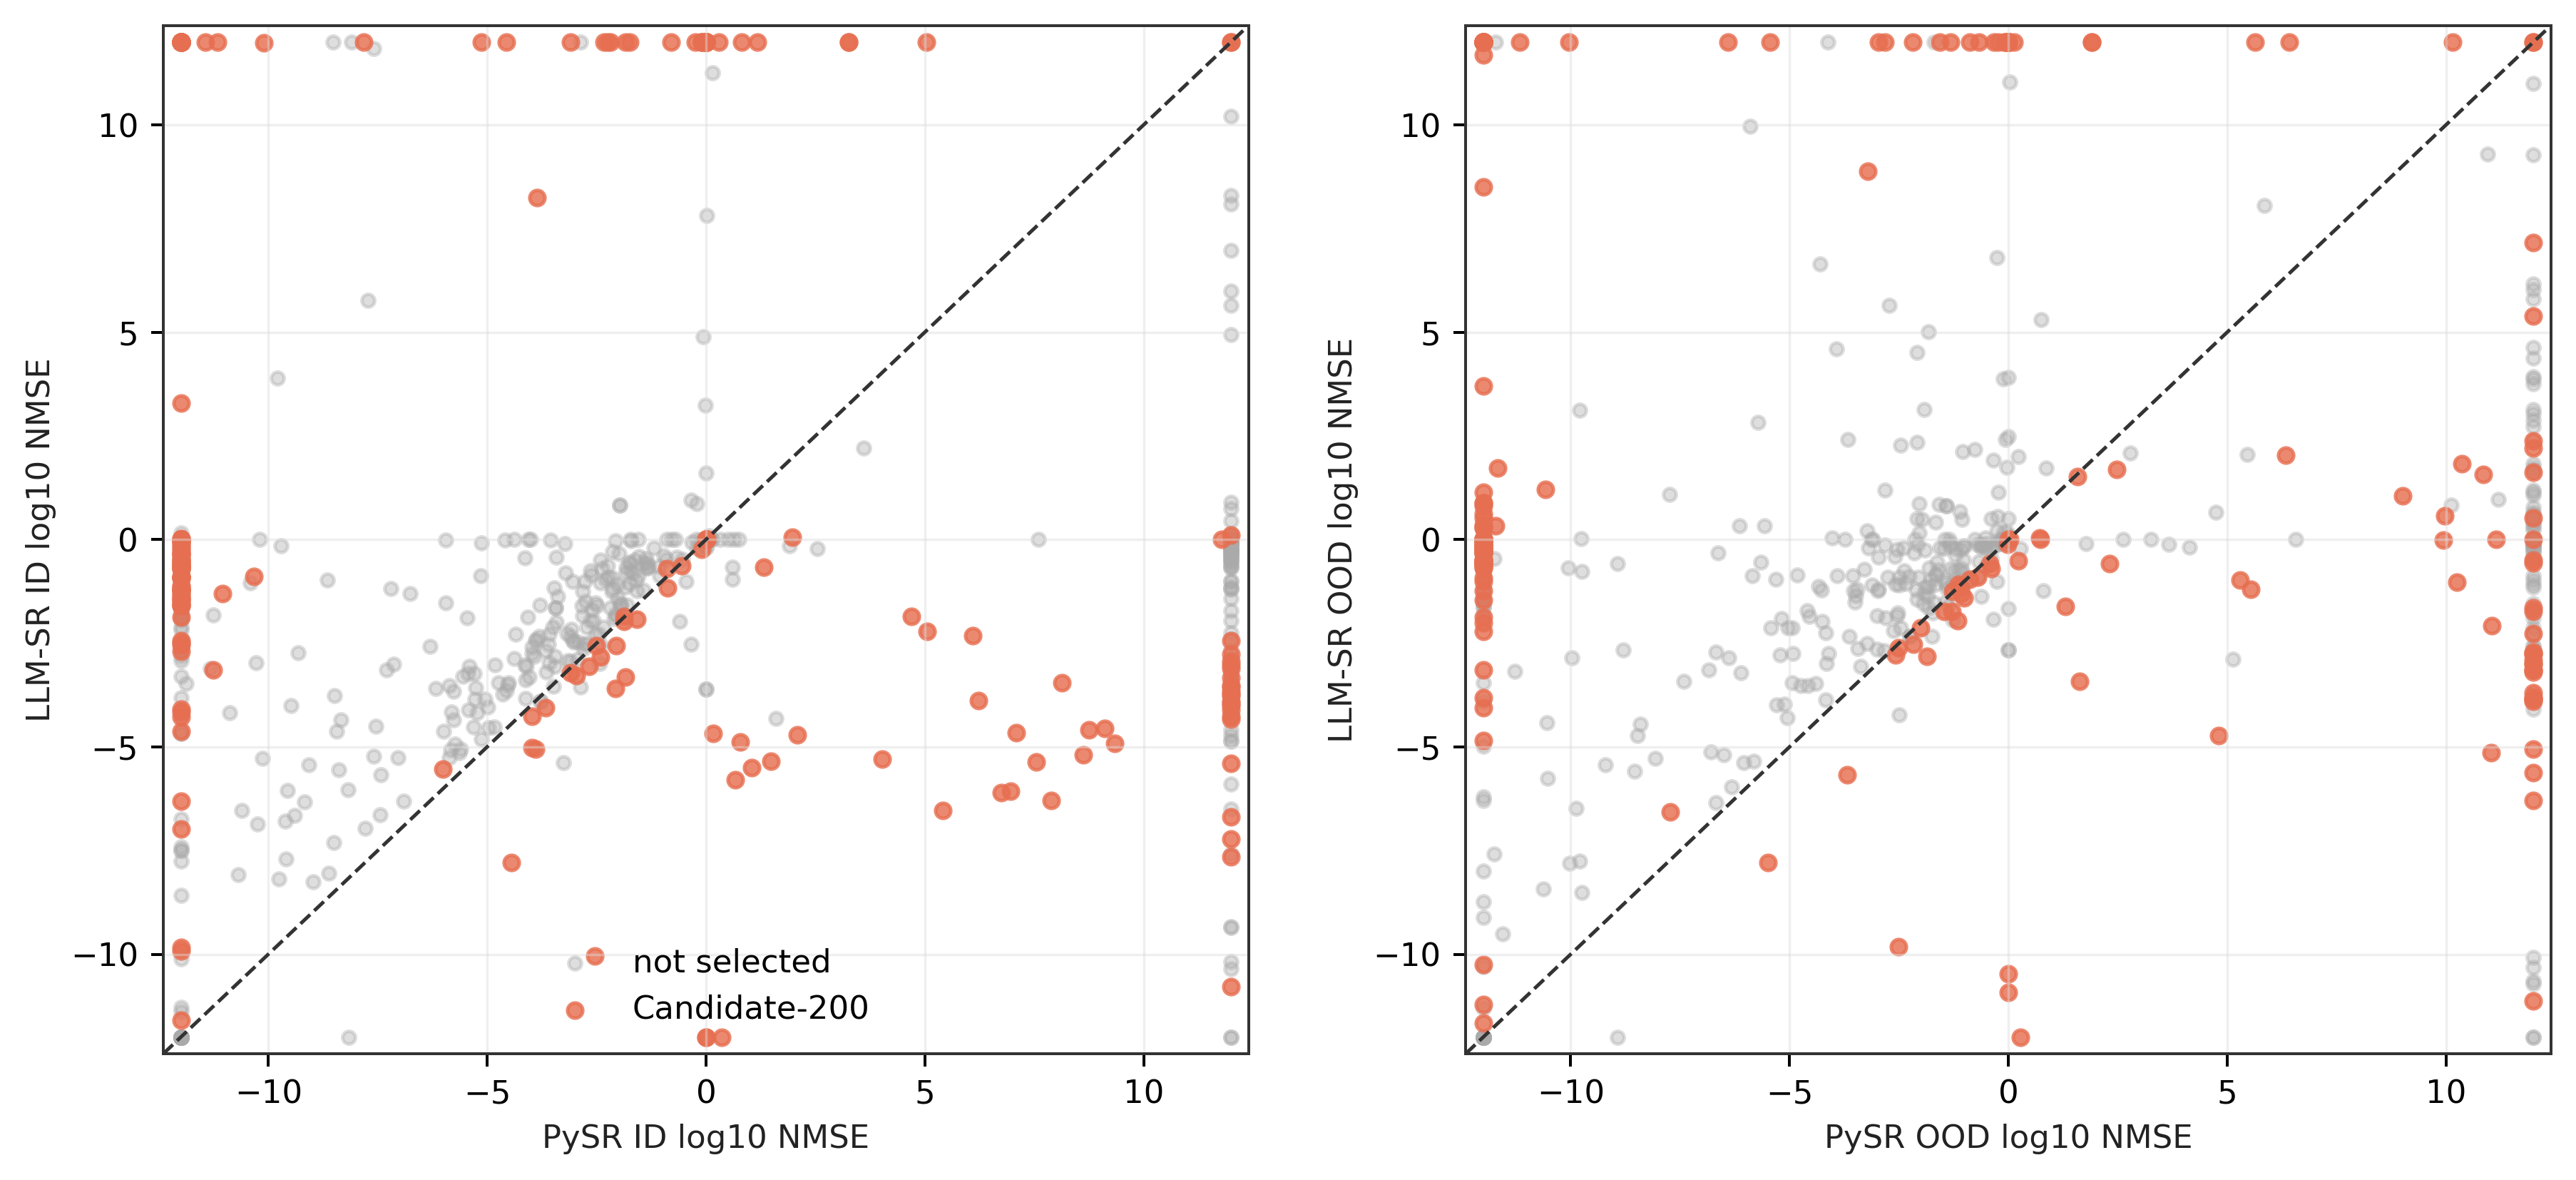
\includegraphics[width=\linewidth]{imgs/Appendix/figure03_dual_probe_scatter}
% \end{minipage}
% \hfill
% \begin{minipage}{0.49\linewidth}
% \centering
% 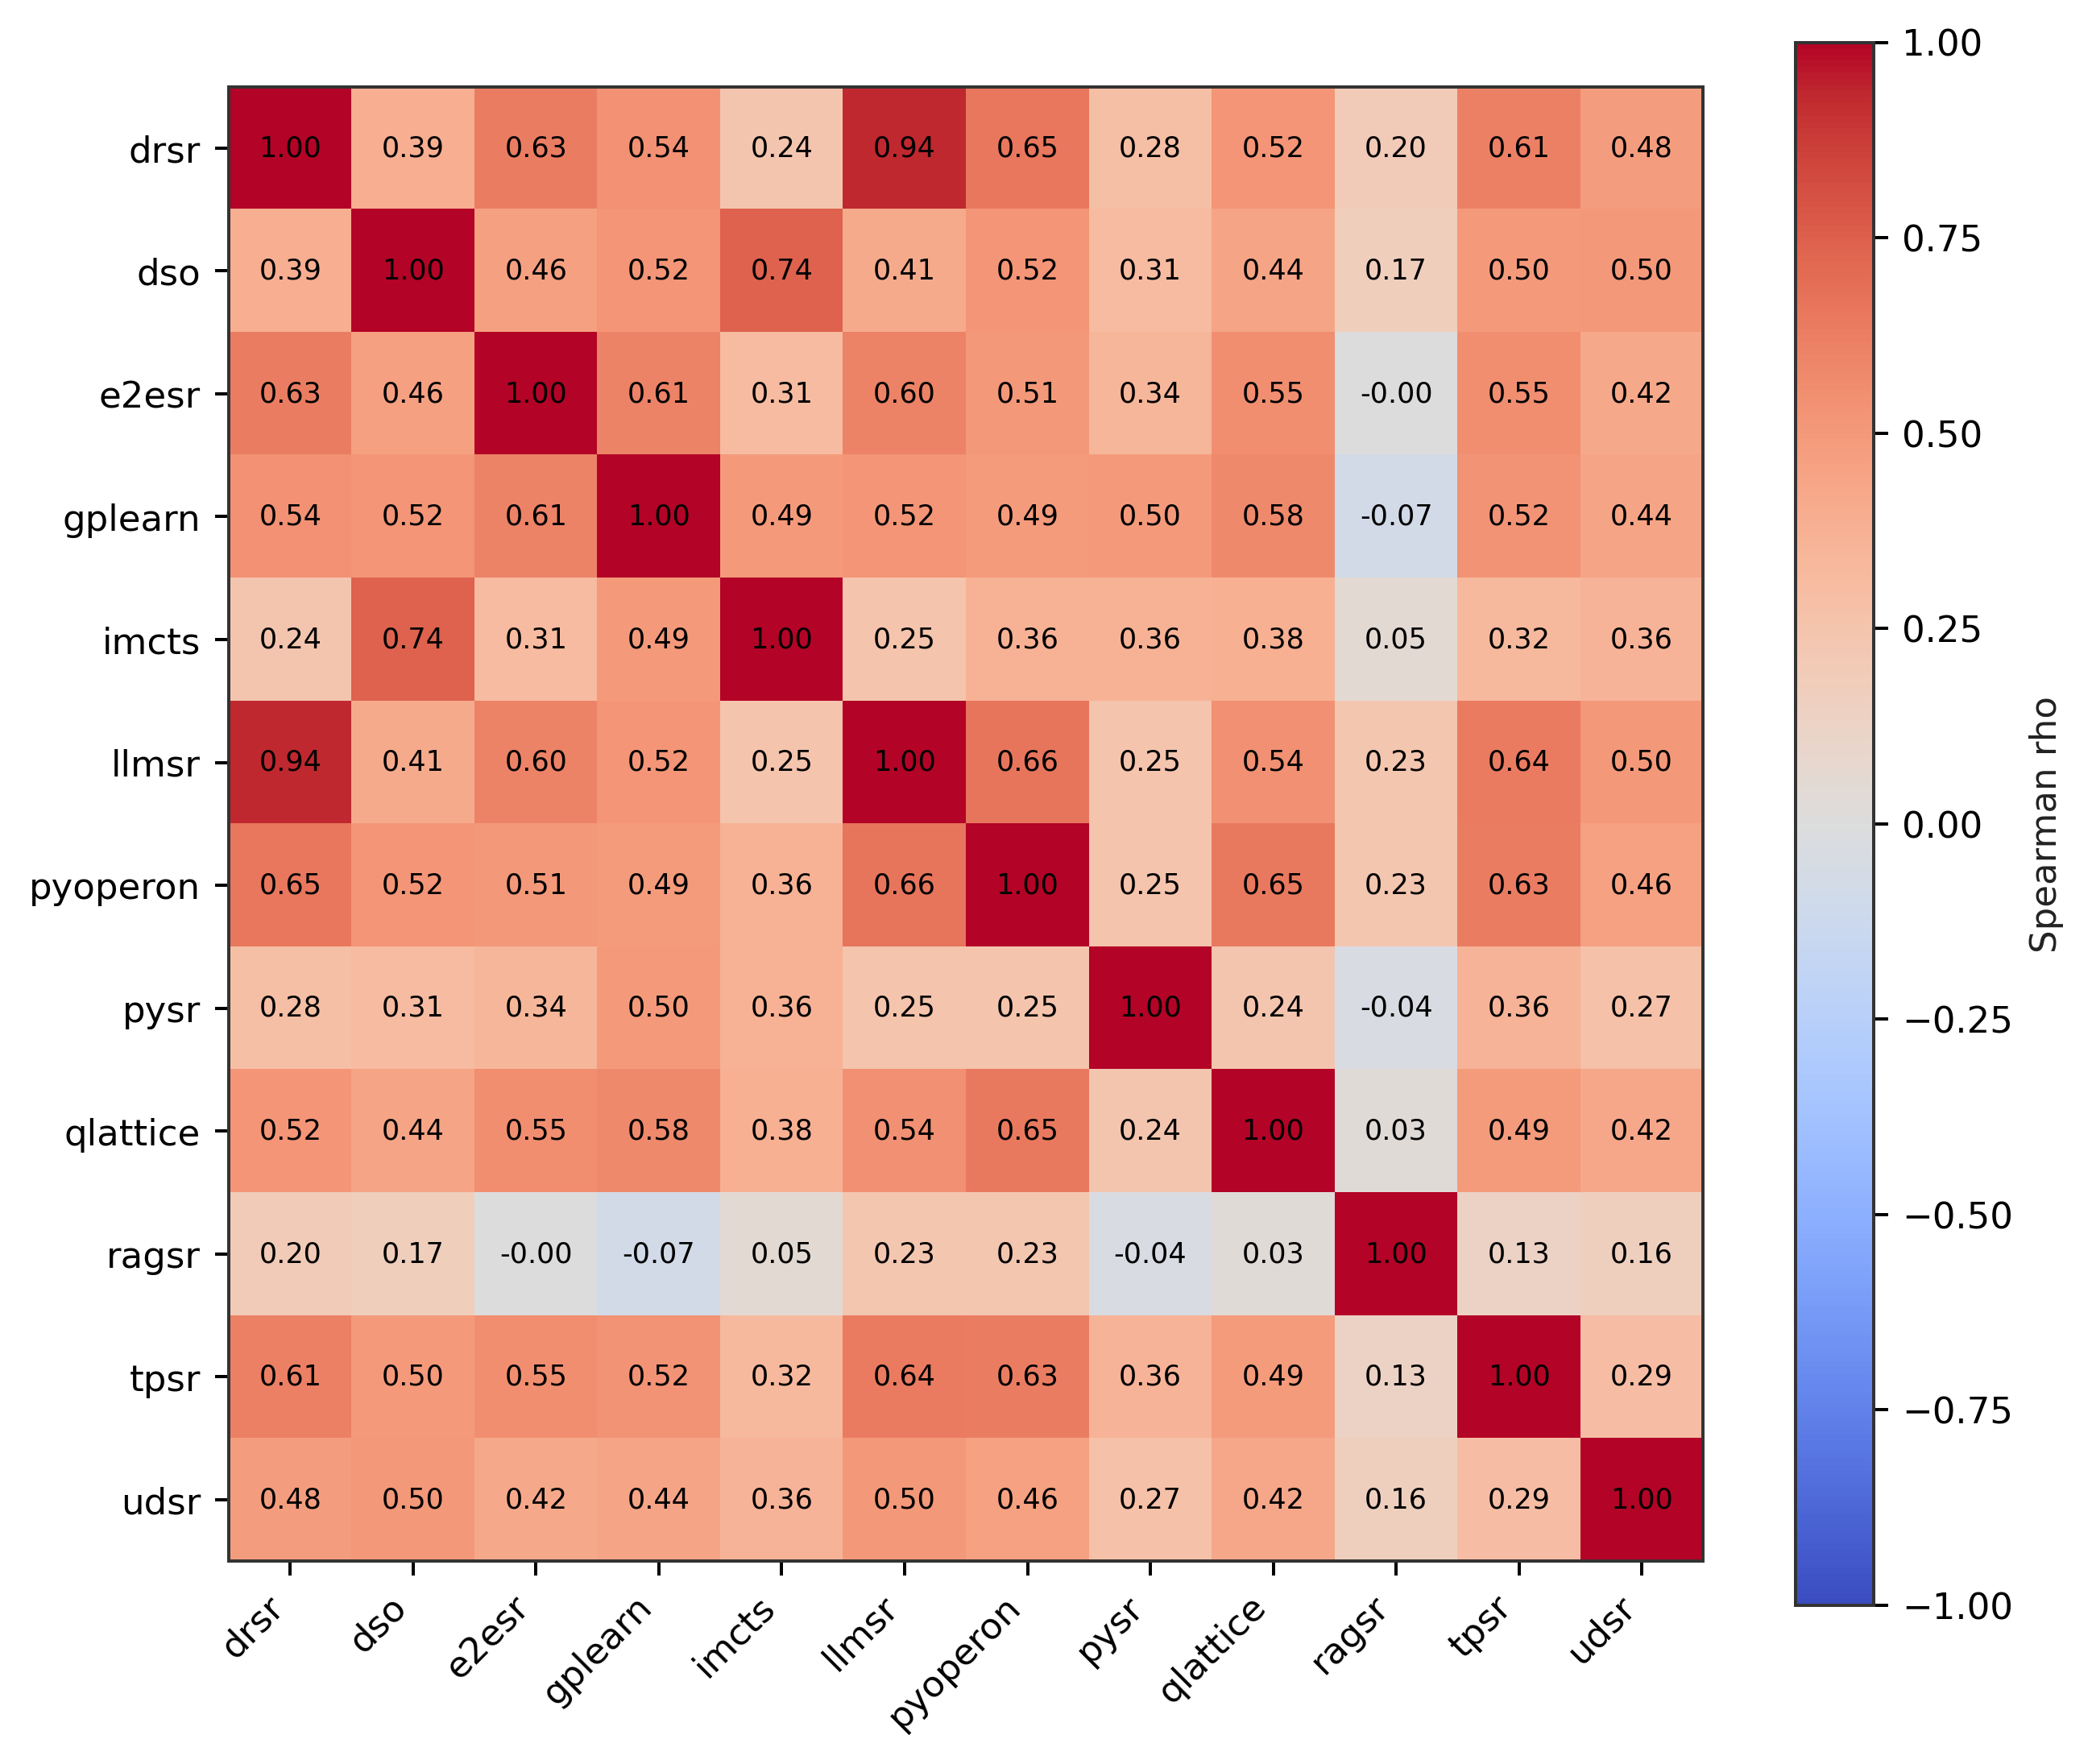
\includegraphics[width=\linewidth]{imgs/Article/figure07_algorithm_behavior_correlation}
% \end{minipage}
% \caption{Distillation diagnostics. Left: PySR/LLM-SR disagreement identifies high-information Candidate-200 regions without using physical background descriptions. Right: response correlation among the 12 calibrated algorithms prevents Probe-4 from collapsing into four redundant methods.}
% \label{fig:distillation-diagnostics}
% \end{figure}

% The final \probe{} is
% \[
% \{\mathrm{DSO}, \mathrm{PyOperon}, \mathrm{iMCTS}, \mathrm{uDSR}\}.
% \]
% This panel is not chosen because it has the highest NMSE-only score. It is chosen because it satisfies the health and taxonomy constraints while remaining a compact surrogate for broader algorithm-panel behavior. \Cref{app:core50-details} reports the top NMSE-only combinations and the final selected panel for auditability.

% \subsection{Probe4-Full response profiles}

% We run \probe{} on all 664 reservoir tasks with three seeds:
% \[
% 664 \times 4 \times 3 = 7968 \text{ runs}.
% \]
% Each run records status, validity, train/validation/ID/OOD metrics, runtime, expression, complexity, and failure reason. NMSE values are converted to clipped log space:
% \[
% \ell(\mathrm{NMSE})=\mathrm{clip}(\log_{10}(\max(\mathrm{NMSE},10^{-12})),-12,12).
% \]
% For each dataset--probe pair, seed-level results are aggregated into median ID/OOD log-NMSE, seed IQR, valid rate, runtime, and complexity. These response profiles are the only result-derived inputs used to score dataset informativeness.

% \subsection{\core{} objective and constraints}

% Each dataset has a structural profile and a Probe-4 response profile. The structural profile contains static metadata such as family, subgroup, semantic duplicate group, feature count, sample scale, formula complexity, operator type, OOD type, and dummy-variable status. The response profile contains Probe-4 median ID/OOD performance, ID-to-OOD degradation, valid-output pattern, winner probe, and seed-level stability.

% The main selection objective is:
% \[
% S^*=\arg\max_{S\subset D,\ |S|=50}
% \left[
% 0.45\,\mathrm{Coverage}(S)
% +0.35\,\mathrm{MeanInfo}(S)
% +0.20\,\mathrm{Balance}(S)
% \right].
% \]
% Here, $\mathrm{Coverage}$ preserves both structural and response-space coverage, $\mathrm{MeanInfo}$ rewards tasks that discriminate between probes while remaining seed-stable, and $\mathrm{Balance}$ penalizes distributional drift from the 664-task reservoir. Dataset information is summarized as
% \[
% \mathrm{Info}_i=\mathrm{Discrimination}_i \times \mathrm{Stability}_i.
% \]
% Intuitively, a high-information dataset is one where the probes behave differently for stable reasons, rather than because of random seeds, invalid outputs, or timeout artifacts.

% Hard constraints prevent the objective from collapsing into a pathological subset. They cap semantic duplicates, basename/source concentration, subgroup concentration, invalid-prone and one-sided cases, and extreme-difficulty cases, while preserving family and difficulty coverage. No source family receives a hand-written special rule: family quotas are derived from reservoir proportions with uniform smoothing. The released manifest also excludes result-derived columns such as probe gap, priority score, and selected advantage side; final benchmark materialization is audited using dataset identity and static metadata only. The detailed coverage map is provided in \cref{app:additional-figures}.

% \subsection{\core{} validation}

% After selection, we validate \core{} against the full reservoir using Probe4-Full results. The validation checks whether the 50-task subset preserves method ranking, pairwise preferences, aggregate scores, and distributional structure from the 664-task reservoir. It also compares \core{} against repeated random and family-stratified subsets, together with curated alternatives such as top-information, metadata-diverse, and difficulty-balanced subsets. The central validation claim is not that 50 tasks replace the full reservoir, but that \core{} is a high-information development benchmark whose conclusions remain aligned with the larger pool.

% \begin{table}[t]
% \centering
% \small
% \caption{\core{} validation against alternative 50-task selectors. Higher is better for all columns. The table complements the aggregate-error and rank-correlation checks in the experiments section.}
% \label{tab:core50-baseline-main}
% \resizebox{\linewidth}{!}{%
% \begin{tabular}{lrrrrrr}
% \toprule
% Subset & Coverage & Mean info & Rank fidelity & Stability & Non-red. & Diff. balance \\
% \midrule
% \core{} & 0.838 & 0.471 & 1.000 & 0.835 & 0.769 & 0.892 \\
% top-info-50 & 0.784 & 0.691 & 1.000 & 0.911 & 0.860 & 0.780 \\
% metadata-diverse-50 & 0.635 & 0.085 & 1.000 & 0.735 & 0.860 & 0.601 \\
% difficulty-balanced-50 & 0.817 & 0.637 & 1.000 & 0.883 & 0.920 & 0.999 \\
% random-50 avg & 0.835 & 0.187 & 0.983 & 0.705 & 0.970 & 0.908 \\
% family-stratified random-50 avg & 0.815 & 0.191 & 0.995 & 0.696 & 0.968 & 0.909 \\
% \bottomrule
% \end{tabular}
% }
% \end{table}

\section{\core{} Distillation}
\label{sec:core50-distillation}

\paragraph{Goal.}
The purpose of \core{} is not to create a small random subset of the reservoir, but to construct a compact benchmark that preserves the main structural coverage and algorithm-response conclusions of \reservoir{} while remaining cheap enough for repeated leaderboard evaluation. We therefore formulate subset construction as a cascaded distillation problem: an 800+ raw task pool is filtered into the 664-task \reservoir{}, mined into a 200-task calibration set, used to select a compact non-LLM probe panel, and finally distilled into the 50-task \core{} benchmark. Full formulas, quota derivations, implementation details, and audit tables are provided in \cref{app:core50-details}.

\paragraph{Candidate-200 mining.}
The first stage uses two complementary probes, PySR and LLM-SR, on all 664 ground-truth tasks, resulting in $664 \times 2 = 1328$ single-seed runs. Physical background descriptions are withheld, so the LLM-based probe cannot directly exploit semantic context. For each dataset, ID and OOD disagreement between the two probes is computed in clipped log-NMSE space. The 200-task \candidate{} set is not obtained by simply taking the top-200 disagreement cases. Instead, it combines high-disagreement tasks, one-sided evaluability cases, and mid-gap tasks under source, subgroup, basename, and advantage-side caps. The resulting pool contains 140 high-discrimination tasks, 20 one-sided evaluability tasks, and 40 mid-gap tasks. Its role is calibration: it exposes method differences and failure modes, but is not used as the final benchmark.

\paragraph{Probe-4 selection.}
We next run the 12 integrated algorithms on \candidate{} with one seed, producing $200 \times 12 = 2400$ calibration runs. The goal is not to choose the four strongest algorithms, but to choose a small non-LLM probe panel that is healthy enough to run at scale, behaviorally complementary, and faithful to the dataset-informativeness judgments of the broader 12-method panel. For a candidate four-method panel \(P\), the selection score is
\[
\mathrm{Score}(P)
=
0.20H(P)
+
0.40F(P)
+
0.25C(P)
+
0.15V(P),
\]
where \(H\) measures execution health, \(F\) measures fidelity to the 12-method panel, \(C\) measures behavioral complementarity, and \(V\) measures dataset coverage. Taxonomy constraints require at least three algorithmic paradigms, and construction-role constraints exclude methods whose behavior depends on LLM/RAG context or whose role is already used in dual-probe mining. The final \probe{} is selected as $\{\mathrm{DSO}, \mathrm{PyOperon}, \mathrm{iMCTS}, \mathrm{uDSR}\}$, yielding a compact surrogate that spans policy search, evolutionary GP, tree search, and neural-guided SR.

% \paragraph{Core-50 construction.}
% The selected \probe{} is evaluated on all 664 reservoir tasks with three seeds: $664 \times 4 \times 3 = 7968$ runs. These Probe4-Full runs define a response profile for each dataset, including median ID/OOD performance, ID-to-OOD degradation, valid-output patterns, and seed stability. Together with static structural metadata, these profiles are used to select \core{}:
% \[
% S^*
% =
% \arg\max_{S\subset D,\ |S|=50}
% \left[
% 0.45\,\mathrm{Coverage}(S)
% +
% 0.35\,\mathrm{MeanInfo}(S)
% +
% 0.20\,\mathrm{Balance}(S)
% \right].
% \]
% Here, \(\mathrm{Coverage}\) preserves both structural and response-space diversity, \(\mathrm{MeanInfo}\) rewards tasks that separate probes for stable reasons, and \(\mathrm{Balance}\) controls difficulty and failure-mode drift from the 664-task reservoir. Hard constraints cap semantic duplicates, basename concentration, subgroup concentration, invalid-prone tasks, one-sided cases, and extreme-difficulty cases. Family quotas are derived from reservoir proportions with uniform smoothing, so no source family receives a hand-written special rule. The constrained objective is optimized by greedy initialization, local swaps, and random restarts.

% Once validated, \core{} is frozen as the official development benchmark. The Probe4-Full results are used only for benchmark construction and are not reused as final leaderboard results. The formal leaderboard is recomputed independently by running all 12 algorithms on the frozen \core{} with five seeds: $12 \times 50 \times 5 = 3000$ formal evaluation runs.
\paragraph{Core-50 construction.}
The selected \probe{} is evaluated on all 664 reservoir tasks with three seeds, resulting in \(664 \times 4 \times 3 = 7968\) Probe4-Full runs. These runs, together with static dataset metadata, are used to select a 50-task subset by optimizing
\[
S^*
=
\arg\max_{S\subset D,\ |S|=50}
\left[
0.45\,\mathrm{Coverage}(S)
+
0.35\,\mathrm{MeanInfo}(S)
+
0.20\,\mathrm{Balance}(S)
\right].
\]
Here, \(\mathrm{Coverage}\) preserves structural and response-space diversity, \(\mathrm{MeanInfo}\) rewards stable probe-discriminative tasks, and \(\mathrm{Balance}\) controls difficulty and failure-mode drift. The optimization is performed under hard constraints on duplicates, family/subgroup concentration, invalid-prone cases, one-sided cases, and extreme-difficulty tasks; full definitions are given in \cref{app:core50-details}.

\paragraph{Validation.}
The selected \core{} is validated against the full 664-task reservoir and five subset-selection baselines: random-50, family-stratified random-50, metadata-diverse-50, top-information-50, and difficulty-balanced-50. The validation checks whether \core{} preserves reservoir-level method ordering, pairwise preferences, aggregate scores, structural distribution, difficulty balance, and failure-mode coverage. After validation, \core{} is frozen, and the final leaderboard is recomputed independently using all 12 algorithms with five seeds, yielding \(12 \times 50 \times 5 = 3000\) formal evaluation runs.
